\documentclass[xcolor=table]{beamer}
\usepackage[UTF8, noindent]{ctexcap}
\usetheme{PaloAlto}
%\usecolortheme{crane}
%\rowcolors{2}{craneorange!25}{craneorange!50}
\rowcolors{2}{gray!25}{gray!50}
\usecolortheme{seagull}

\usepackage{arev}
\usepackage{amsmath}
\usepackage{tikz}
\newtheorem{thm}{定理}
\bibliographystyle{apalike}
\logo{\includegraphics[scale=0.5]{res/logo4.pdf}}

\title{杂谈勾股定理}
\subtitle{数学史讲座之一}
\institute{九章学堂}
\author{张三}
\date{\today}
\subject{勾股定理}
\keywords{勾股定理,历史}

\begin{document}

%\maketitle
\begin{frame}
\titlepage
\end{frame}

\begin{frame}{目录}
\tableofcontents
\end{frame}

\section{勾股定理在古代}

\begin{frame}{古希腊数学}
勾股定理在西方称为毕达哥拉斯定理,古希腊数学家在 2000 多年前就已经发现并证明了它\cite{Kline}。
\begin{itemize}
\item 公元前 6 世纪,毕达哥拉斯学派发现了一个法则,可以构造直角三角形的边长;
\item 公元前 3 世纪,欧几里德《几何原本》使用面积法证明勾股定理。
\end{itemize}
\end{frame}

\begin{frame}{古中国数学}{定理发现}
中国在 3000 多年前就知道勾股数的概念,比古希腊更早一些。

《周髀算经》的记载:
\begin{itemize}
\item 公元前 11 世纪,商高答周公问:
\begin{quote}
勾广三,股修四,径隅五。
\end{quote}
\item 又载公元前 7--6 世纪陈子答荣方问,表述了勾股定理的一般形式:
\begin{quote}
若求邪至日者,以日下为勾,日高为股,勾股各自乘,并而开方除之,得邪至日。
\end{quote}
\end{itemize}
\end{frame}

\begin{frame}{古中国数学}{定理证明}
有论者认为早在公元前 11 世纪商高即已证明勾股定理\cite{quanjing}。
完整的证明见于三国时(公元 3 世纪)赵爽对《周髀算经》的注释。
\begin{figure}
   \centering
   \includegraphics[scale=0.3]{res/xiantu.pdf}
   \caption{赵爽的弦图可给出了勾股定理的一个富于对称美的证明}
\end{figure}

\end{frame}


\section{勾股定理在现代}
\begin{frame}{现代叙述}
\begin{thm}[勾股定理]
直角三角形斜边的平方等于两腰的平方和。

可以用符号语言表述为:设直角三角形 ABC,其中 $\angle$C = 90$^\circ$,则有
\begin{equation}\label{eq:gougu}
AB^2=BC^2+AC^2
\end{equation}
\end{thm}
\begin{center}
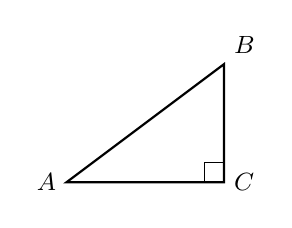
\begin{tikzpicture}[scale=0.5,font=\small]
\draw[thick] (0,0) node[left] {$A$}
    -- (4,0) node[right] {$C$}
    -- (4,3) node [above right] {$B$} -- cycle;
\draw (3.5,0) |- (4,0.5);
\end{tikzpicture}
\end{center}
\end{frame}

\begin{frame}{勾股数}
满足式\eqref{eq:gougu}的整数称为\emph{勾股数}。第1节所说毕达哥拉斯学派得到的三元数组就是勾股数。下表列出一些较小的勾股数:
\begin{table}[H]
\begin{tabular}{rrr}

%\rowcolor{craneorange}
\rowcolor{gray}
直角边 $a$ & 直角边 $b$ & 斜边 $c$\\

3 & 4 & 5 \\
5 & 12 & 13 \\
7 & 24 & 25 \\
8 & 15 &17 \\

\end{tabular}
\caption{较小的几组勾股数}
\end{table}
\end{frame}

\begin{frame}{参考文献}
\nocite{Shiye}
\bibliography{bib/newmath}
\end{frame}

\end{document}
